%
% fresnel-c-s-komplex.tex -- C-S-Plot
%
% (c) 2021 Prof Dr Andreas Müller, OST Ostschweizer Fachhochschule
%
\documentclass[tikz]{standalone}
\usepackage{amsmath}
\usepackage{times}
\usepackage{txfonts}
\usepackage{pgfplots}
\usepackage{csvsimple}
\usetikzlibrary{arrows,intersections,math,calc}
\definecolor{darkred}{rgb}{0.8,0,0}
\definecolor{darkgreen}{rgb}{0,0.6,0}
\begin{document}
\def\skala{1}
\begin{tikzpicture}[>=latex,thick,scale=\skala]

\clip (-4.7,-4.8) rectangle (5.7,5.02);
\node at (0,0) {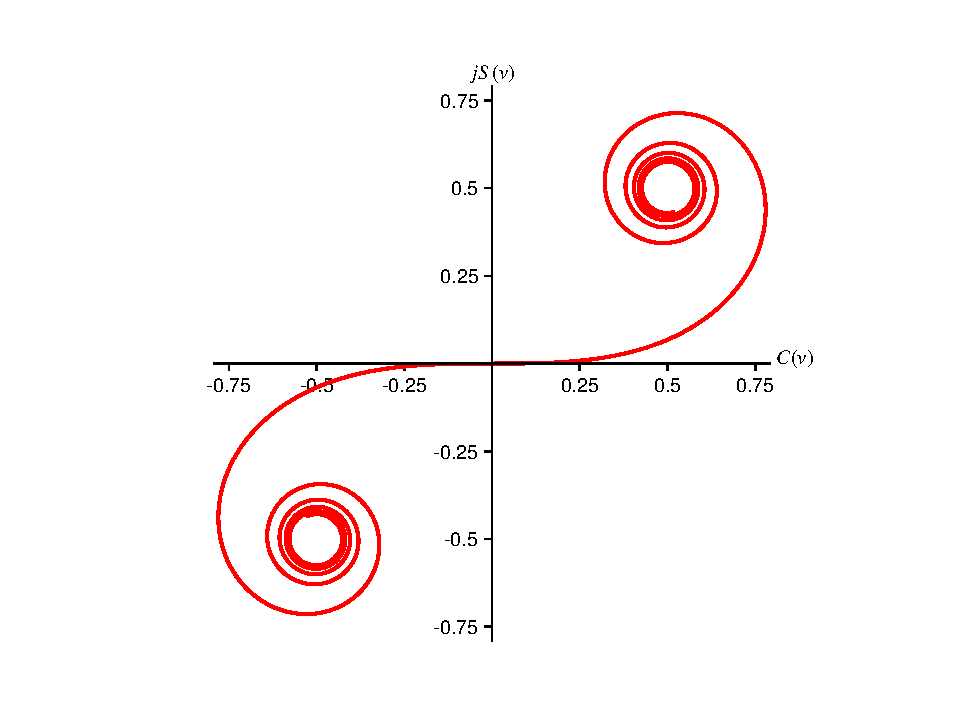
\includegraphics{cs-komplex.pdf}};

\end{tikzpicture}
\end{document}

